Как было показано на нескольких примерах в разделе~\ref{sec:resonance}, в двух- 
и трех-вершинных процессах сингулярность в амплитудах возникает в пропагаторах 
виртуальных частиц, которая устраняется введением конечной ширины резонансного 
пика, определяемой мнимой частью знаменателя пропагатора виртуальной частицы. С 
другой 
стороны, для одновершинных реакций, таких как однофотонное 
рождение электрон-позитронной пары $\gamma\to e^+e^-$ или поглощение фотона 
$e^{\pm}\gamma\to e^{\pm}$, которые кинематически запрещены или подавлены в 
вакууме, но становятся возможными в присутствии активной среды, при 
определенных энергиях участвующих частиц тоже возникают 
расходимости в вероятностях процессов, связанные со свойствами фазового объема 
(см., 
например,~\cite{Klepikov:1954,Sturrock:1971,Tademaru:1973,Daugherty:1983,Shabad:1988}).
В отличие от двухвершинных процессов, ввести ширину резонансного пика на основе 
мнимой части знаменателя пропагатора невозможно в виду его отсутствия для 
одновершинного процесса.  При расчетах 
физических величин все резонансные бесконечные пики 
усреднялись~\cite{Baier:2007}, что позволило получить конечные результаты, 
однако такой подход не устраняет сингулярности, поэтому требуется 
переформулировать модель в других терминах. 

Чтобы устранить эти сингулярности, в работе~\cite{Shabad:1988} было предложено  
рассматривать фотон как затухающую электромагнитную волну, то есть исследовать 
временную зависимость волновой функции фотона.
При ее учете возникает мнимая часть поляризационного оператора фотона, которая 
определяет коэффициент затухания электромагнитной волны, что приводит к 
конечной ширине резонансного пика.

Изначально классическая задача о диссипации электромагнитной волны  в 
бесстолкновительной плазме 
рассматривалась в работе~\cite{Landau:1946}, что в последствии получило 
название затухание Ландау. Если в классической задаче затухание связано либо с 
передачей энергии электромагнитного поля частицам, движущимся в фазе с волной, 
либо с ларморовым вращением частиц, то в квантовой электродинамике затухание 
электромагнитной волны определяется процессами 
поглощения и рождения фотонов. Особенностью рассмотренных выше классических и 
квантовых процессов является их обратимость.

Для поиска временной зависимости волновой функции фотона в 
работе~\cite{Shabad:1988} предлагалось решать уравнение дисперсии на втором 
римановом листе. Однако, как было отмечено в работе~\cite{MikhChist:2001}, 
такой метод имеет ряд недостатков. Во-первых, решения с комплексными энергиями 
фотона находятся на нефизических римановых листах, количество которых, вообще 
говоря, бесконечно. Это приводит к возникновению бесконечного числа решений 
уравнения дисперсии как с положительными, так и с отрицательными значениями 
мнимой части энергии. Во-вторых, в данном методе в околопороговой области 
предполагался экспоненциальный характер затухания электромагнитной волны, что 
согласно выводам авторов~\cite{MikhChist:2001}, не так. Поэтому 
в работе~\cite{MikhChist:2001} для исследования временного затухания 
электромагнитной волны во внешнем магнитном поле был рассмотрен метод, который 
заключается в нахождении запаздывающего решения уравнения электромагнитного 
поля в присутствии внешнего источника с учетом поляризации вакуума во внешнем 
магнитном поле. С другой стороны, в работе~\cite{MikhChist:2001} 
неэкспоненциальное затухание фотона рассматривалось в приближении сильного 
магнитного поля, когда все электроны и позитроны занимают основной уровень 
Ландау, однако в случае замагниченной плазмы таких исследований не проводилось, 
поскольку для астрофизических приложений наличие замагниченной среды является 
наиболее характерным фактором.


%So the probability diverges when
%the electron and the positron are created on the Landau
%levels with electron and positron momentum p3  0, see
%e.g. [6,10]. The origin of the singularity is due to the
%properties of the space volume in the lowest order of
%perturbation theory (infinitesimally narrow level). The reason why this singularity is not a pole but a branch point is
%that motion along a field is not quantized.

В данной главе рассматривается затухание фотона в сильно замагниченной плазме, 
$\beta 
\gg T^2$,
 с нулевым химическим потенциалом, $\mu = 0$, посредством изменения его 
 состояния 
за счет процессов $\gamma e^\pm\to e^\pm$, $\gamma \to e^+e^-$. Будет 
использоваться метод, применяемый в теории поля при конечных температурах и в 
физике плазмы~\cite{Boyan}, развитый на случай сильного магнитного поля 
в~\cite{MikhChist:2001} и адаптированный к ситуации сильно замагниченной плазмы.

\subsection{Распространение фотона в замагниченной плазме}

Для описания эволюции электромагнитной волны ${\cal A}_{\alpha}(x)$ 
во времени воспользуемся методикой, которая была предложена еще в классической 
задаче~\cite{Landau:1946} и развита  в работе~\cite{MikhChist:2001} для 
квантовой электродинамики с учетом только магнитного поля без плазмы. Данная 
методика заключается в определении реакции системы 
(${\cal A}_{\alpha}(x)$ и замагниченной плазмы) на внешний источник~\cite{Kirzhnits:1987}, создающий начальное состояние, который адиабатически включается 
при $t = - \infty$ и в момент времени $t = 0$ выключается. При $t > 0$
электромагнитная волна в плазме будет эволюционировать самостоятельно. Для простоты будем рассматривать эволюцию монохроматической волны, поэтому 
функцию источника, удовлетворяющую вышесказанным условиям, удобно выбрать следующим образом:
%
\beq
{\cal J}_{\alpha}(x) = j_{\alpha}\,e^{i \,{\bf k} {\bf x}}\,
e^{ \varepsilon t}\, \theta(- t), \,\,\, \varepsilon \to 0^+,
\label{eq:1}
\eeq
где $j_{\alpha} = (0, {\bf j}),\,\,{\bf j} \cdot {\bf k} = 0$ – закон 
сохранения тока. Вообще говоря, в замагниченной плазме из-за наличия 
анизотропии решение задачи о распространении фотона под произвольным углом к 
магнитному полю представляет значительные трудности. Поэтому в качестве 
упрощения рассмотрим частный случай, когда фотоны распространяются поперек 
магнитного поля так, что $k_z=0$. Зависимость ${\cal A}_{\alpha}(x)$ от 
времени  определяется уравнением:
%
\begin{eqnarray}\label{eq:WaveEq5}
%\nonumber
%&& 
(g_{\alpha \beta} \, \partial_{\mu}^2  -
\partial_{\alpha}\partial_{\beta}) \, {\cal A}_{\beta}(x) + 
%\nonumber \\
%&&+ 
\int d^4 x'\, {\cal P}_{\alpha \beta} (x - x') \, {\cal A}_{\beta}(x')
= {\cal J}_{\alpha}(x),
\label{eq:2}
\end{eqnarray}
%                                                                                         \frac{(\varphi q)_\mu}{\sqrt{q^2_\perp}}
где ${\cal P}_{\alpha \beta} (x - x')$ -- поляризационный оператор фотона в 
магнитном поле и плазме (см. главу~\ref{Ch:Photon}).

% Следует отметить, что в общем случае поляризационный оператор зависит от каждой координаты $x$ и $x'$ в отдельности. Однако, если рассматриваются процессы на достаточно малых расстояниях и временах, то среду в таком случае можно считать однородной. Тогда поляризационный оператор будет зависеть от разности $x-x'$.


Запаздывающее решение уравнения~(\ref{eq:WaveEq5}) можно представить в 
следующем виде:

\begin{equation}\label{eq:RetSol}
	{\cal A}_\alpha(x)=\int \dd^4 x' G^R_{\alpha \beta}(x-x'){\cal J}_\beta(x')\, ,
\end{equation}
где $G^R_{\alpha \beta}(x-x')$ -- запаздывающая функция Грина (см., например~\cite{Landau:2001}).

Следуя работе~\cite{MikhChist:2001}, аналогично процессу затухания в магнитном 
поле, воспользуемся следующим соотношением между запаздывающей 
$G^R_{\alpha\beta}(x-x')$ и причинной $G^C_{\alpha\beta}(x-x')$ функциями Грина:

\begin{equation}\label{eq:RetCasualGreen}
G^R_{\alpha\beta}(x-x')= 2 \mathrm{Re} \left[G^C_{\alpha\beta}(x-x')\right]\theta(t-t')\, .
\end{equation}

Разложение функции Грина по собственным векторам 
$r_\alpha^{(\lambda)}$ поляризационного оператора в замагниченной плазме 
выглядит следующим образом:
\begin{equation}\label{eq:InvGcFourier}
	G^C_{\alpha\beta}(x)=\int \frac{\dd^4q}{(2\pi)^4}G^C_{\alpha \beta}(q) e^{-\ii qx}\, ,
\end{equation}
\begin{equation}\label{eq:GcFourier}
	G^C_{\alpha\beta}(q)=\sum_{\lambda=1}^{3}\frac{r_\alpha^{(\lambda)}r^{(\lambda)}_\beta}{(r^{(\lambda)})^2}\cdot
	 \frac{1}{q^2-{\cal P}^{(\lambda)}(q)}\, .
\end{equation}


В силу линейного характера уравнения~(\ref{eq:WaveEq5}), 
решение для двух возможных поляризаций (см. 
главу~\ref{Ch:Photon}) можно представить в виде:
\begin{equation}\label{eq:ASoveDivide}
	{\cal A}_\alpha(x)={\cal A}^{(1)}_\alpha(x)+{\cal A}^{(2)}_\alpha(x)\, ,
\end{equation}
где 
%
\begin{eqnarray}\label{eq:ASoveF}                     		
{\cal A}^{(\lambda)}_{\alpha} (x) = V^{(\lambda)}_\alpha (0, {\bf x}) \, \text{Re} F^{(\lambda)} (t) \, ,
\label{eq:V}
\end{eqnarray}
\begin{eqnarray}
V^{(\lambda)}_\alpha (0, {\bf x}) = 2\, e^{ i\, {\bf k x}} \, 
\varepsilon^{(\lambda)}_\alpha \, (\varepsilon^{(\lambda)} j)\, .
\label{eq:partialV}
\end{eqnarray}
%
%\beq
%V^{(2)}_\alpha (0, {\bf x}) = 2\, e^{ i\, {\bf k x}} \, \varepsilon^{(2)}_\alpha \, \frac{(q \tilde \varphi j)}{\sqrt{q^2_{\mprl}}} \, .
%\label{eq:partialV2}
%\eeq
%Для дальнейшего анализа, контур интегрирования удобно
%преобразовать в контур, изображенный на рис.11. 

Как следует из~(\ref{eq:ASoveF}), характер распространения фотона в сильно 
замагниченной плазме будет полностью определяться функцией $F^{(\lambda)} (t)$, 
которая имеет следующий вид Фурье-интеграла:

\begin{equation}\label{eq:FullIntegrate}
	F^{(\lambda)}(t)=\int\limits_{C}\frac{dq_0}{2\pi \ii}\frac{e^{-\ii q_0 
	t}}{(q_0-\ii \varepsilon)(q_0^2-\vec{k}^2-{\cal P}^{(\lambda)}(q))}.
\end{equation}



Контур интегрирования $C$ определяется согласно аналитическим свойствам подынтегрального выражения. В частности, в точке $q_0=\omega$ подынтегральное выражение~(\ref{eq:FullIntegrate}) имеет полюс, который соответствует уравнению дисперсии:
\begin{equation}
	\omega^2 - \vec{k}^2 - {\cal P^{(\lambda)}}(q)=0.
\end{equation}

\begin{center}
	\begin{figure}[t!]\centering
		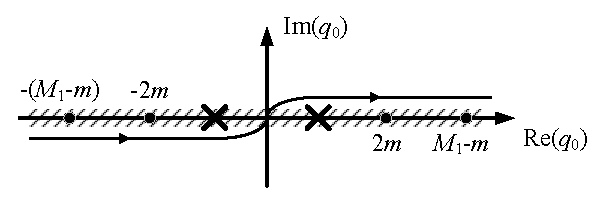
\includegraphics[scale=1.5]{PathIntegrateMode2.eps}
		\caption{Контур интегрирования по $q_0$ в~(\ref{eq:FullIntegrate}) для мод $\lambda =1,2$. Штрихами показана область нестабильности фотона. Крестиком 
		обозначен полюс, соответствующий $q_0=\omega$ -- вещественному 
		собственному значению поляризационного оператора, точками обозначены 
		полюса для моды 2.} \label{fig:FullPathIntegrMode1}
	\end{figure}
\end{center}

С другой стороны, как было показано в работе~\cite{MikhChist:2001}, собственные значения поляризационного оператора как в магнитном поле, так и в замагниченной плазме помимо полюсов $q_{\mprl}^2=(M_n\pm M_\ell)^2$, отмеченных в разделе~\ref{Ch:Compton}, также имеют разрезы, которые связаны с распадом фотона на $e^+e^-$-пару и переходом электрона на другие уровни Ландау, т. е. соответствуют областям нестабильности фотона, поэтому с учетом этих особенностей  контур интегрирования может быть определен, как показано на~рис.~\ref{fig:FullPathIntegrMode1}.

Следует отметить, что в сильно замагниченной плазме в кинематической области $q_0<2m$ мнимая часть поляризационного оператора для обеих мод пренебрежимо мала по сравнению с реальной частью (влияние резонансов отсутствует), поэтому для удобства контур интегрирования как для фотона моды~1, так и для фотона моды 2 можно преобразовать согласно рис.~\ref{fig:PathIntegr}. Таким образом, интеграл~(\ref{eq:FullIntegrate}) можно представить в виде двух слагаемых
\begin{eqnarray}
F^{(\lambda)}(t) = F^{(\lambda)}_{pole}(t) + F^{(\lambda)}_{cut}(t),
\label{eq:19}
\end{eqnarray}
%
первое из которых определяется вычетом в точке $q_0 = \omega$, являющейся
решением уравнения дисперсии $q^2 - {\cal P}^{(\lambda)}(q) = 0$ в кинематической области, где собственное 
значение поляризационного оператора фотона ${\cal P}^{(\lambda)}(q)$ 
вещественно. 

%Оно соответствует незатухающему
%решению в области $\omega < 2 m$~\cite{Shab}.
Второе слагаемое определяет зависимость потенциалов ${\cal A}^{(\lambda)}_\alpha(x)$ от времени
в области $q_0>2m$ и имеет вид
фурье-интеграла:
%
\begin{eqnarray}
F^{(\lambda)}_{cut}(t) &=& \int \limits_{- \infty}^{\infty} \frac{dq_0}{2 \pi}\,
F^{(\lambda)}_{cut}(q_0)e^{- i q_0 t},
\label{eq:20} 
\\
F^{(\lambda)}_{cut}(q_0) &\simeq& 
\frac{2 \,\theta (q_0  -  2 m)\,\text{Im}{\cal 
		P}^{(\lambda)}(q_0 + i \varepsilon)}
{q_0\,([ q_0^2 - {\bf k}^2 - \text{Re} {\cal P}^{(\lambda)}(q_0)]^2 + 
[\text{Im}{\cal 
P}^{(\lambda)}(q_0 + i \varepsilon)]^2)}.
\label{eq:21}
\end{eqnarray}

Мнимая часть поляризационного оператора может быть получена из коэффициента  
поглощения фотона, который имеет следующий вид:
\begin{eqnarray}
W^{(\lambda)}_{abs} = W_{\gamma^{(\lambda)} \to e^+ e^-} + 
W_{\gamma^{(\lambda)} e^{\pm} \to e^{\pm}} \, ,
\label{eq:Wabs}
\end{eqnarray}
где $W_{\gamma^{(\lambda)} \to e^+ e^-}$ -- коэффициент поглощения фотона в процессе однофотонного рождения электрон-позитронной пары, $W_{\gamma^{(\lambda)} e^{\pm} \to e^{\pm}}$ -- коэффициент поглощения фотона в процессе поглощения фотона электроном.

\begin{figure}[t]\centering
	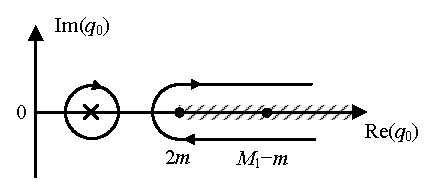
\includegraphics[scale=1.5]{PathIntegrate2Gl.eps}
	\caption{Контур интегрирования по $q_0$ в~(\ref{eq:20}) для мод $\lambda = 1,2$. Штриховой линией показана область, где мнимая часть поляризационного оператора двух возможных мод $\lambda = 1,2$ существенна. Остальные обозначения аналогичны~рис.~\ref{fig:FullPathIntegrMode1}.}\label{fig:PathIntegr}
\end{figure}

С учетом процессов излучения фотонов мнимая часть поляризационного оператора 
может быть представлена в 
следующей форме (см., например,~\cite{Shabad:1988, 
Rumyantsev:2017,Weldon:1983}): 
\begin{eqnarray}\label{eq:Ilambda}
\text{Im} {\cal P}^{(\lambda)} =  -2 q_0 [1-\exp (-q_0/T)] W^{(\lambda)}_{abs} 
\, . 
\label{eq:ImP}
\end{eqnarray}

Реальная часть 
поляризационного оператора может быть восстановлена по его мнимой части с помощью дисперсионного соотношения с одним 
вычитанием:
%
\beq 
\textrm{Re}{\cal P}^{(\lambda)} (t) = \int \limits_0^\infty 
\frac{\textrm{Im}({\cal P}^{(\lambda)} (t'))\,dt'}{t'-t-i o} - \textrm{Re}{\cal 
P}^{(\lambda)} (0)\,, \qquad  t = q^2_0 \, .
\label{eq:Disp}
\eeq

Следует отметить, что в поставленной задаче рассматриваются процессы только до 
второго циклотронного резонанса, $q_0=M_1-m$, поэтому те же процессы с другими 
уровнями Ландау вклада не дают.
Выражения (\ref{eq:20})-(\ref{eq:Wabs}) с учетом (\ref{eq:Disp}) решают задачу 
о нахождении временной зависимости волновой функции фотона  в присутствии сильно 
замагниченной плазмы. 

В работе~\cite{Shabad:1988}
предполагался экспоненциальный характер затухания с декрементом затухания, 
равным мнимой части энергии фотона, полученным из решения уравнения дисперсии 
на втором римановом листе. Рассмотрение  аналитических свойств Фурье-образа 
$F^{(\lambda)}_{cut}(q_0)$ показывает, что характер временного затухания 
волновой функции в общем случае является неэкспоненциальным. Тем не менее на 
протяжении некоторого характерного отрезка времени $(\sim 
[W^{(\lambda)}_{abs}]^{-1})$
зависимость волновой функции от времени можно приближенно описать как 
экспоненциально затухающие гармонические колебания:
%
\begin{equation}\label{eq:ApproxA}
{\cal A}^{(\lambda)}_\mu(t) \sim e^{- \gamma^{(\lambda)}_\text{eff} \, t/2} \cos 
(\omega^{(\lambda)} t + \phi_0).
\end{equation}
%
Здесь $\omega^{(\lambda)}$ и $\gamma^{(\lambda)}_\text{eff}$ -- эффективная 
частота и коэффициент  
поглощения фотона моды $\lambda$ соответственно, которые должны быть найдены с использованием 
(\ref{eq:20})--(\ref{eq:Wabs}) для каждого значения импульса ${\bf k}$, что определяет эффективный 
закон дисперсии фотона в области его нестабильности.


\subsection{Численный анализ}


\begin{figure}[t]\centering
	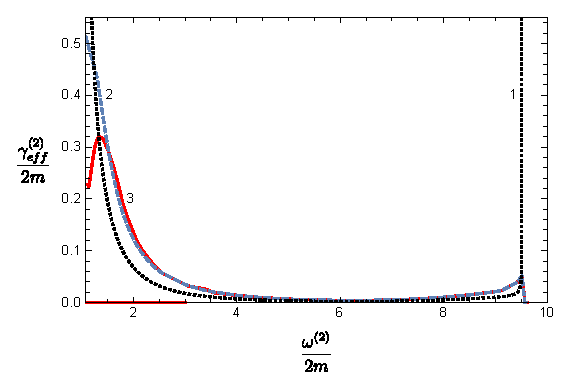
\includegraphics[scale=0.8]{mode2.eps}
	\caption{\label{fig:fig2}Зависимость ширины распада фотона моды 2 от частоты в припороговых областях при $B=200 B_e$, $T=1$ МэВ и $ \mu=0 $. Линия $ {\it 1} $ - коэффициент поглощения фотона $ W ^ {(1)}_{abs} $,
		% в процессах $ \ gamma \ to e ^ + e ^ - $ и $ \ gamma e ^ { \ pm} \ to e ^ {\ pm} $,
		вычисленный в древесном приближении и содержащий корневые особенности; линия $ {\it 2} $ -- ширина распада, полученная из комплексного решения дисперсионного уравнения на втором римановом листе~\cite{Shabad:1988}; линия $ {\it 3} $ соответствует ширине затухания $ \gamma^{(1)}$, вычисленной на основе приближения~(\ref{eq:ApproxA}).}\label{fig:DampMode2}
\end{figure}

Для астрофизических приложений полезно вычислить величину $\gamma_\text{eff}$, которая определяет интенсивность поглощения 
$\gamma$-квантов в замагниченной плазме за счет  процессов $\gamma \to e^+ 
e^-$  и $\gamma e^{\pm} \to e^{\pm}$. На рисунках \ref{fig:DampMode2} 
и~\ref{fig:DampMode1} представлен коэффициент поглощения фотона в зависимости 
от эффективной частоты, определенный исходя из результатов~\cite{Shabad:1988}, 
~\cite{Klepikov:1954} и~\cite{YarkovPhotDampPAN:2022}. 
Анализ показывает, что учет
неэкспоненциального характера 
затухания приводит к конечному выражению для коэффициента  поглощения фотона в окрестности резонансов 
$q_0 = (\sqrt{m^2+2 \beta} - m )$ как для фотона моды 2, так и для фотона моды 
1. Исходя из рис. \ref{fig:DampMode1} можно сделать вывод, что фотон моды 1 
является квазистабильным в областях $q_0<7$ МэВ и $q_0>(\sqrt{m^2+2 \beta} - 
m)\simeq 9.5$~МэВ. С другой стороны, фотон неустойчив в области, близкой в 
окрестности резонанса $q_0 = (\sqrt{m^2+2 \beta} - m )$. Фотон моды 2 можно 
считать квазиустойчивым в области $q_0<4m$ и $q_0>(\sqrt{m^2+2 \beta} - m)$. 
Коэффициент затухания фотона, полученный из результатов 
работы~\cite{Shabad:1988}, является завышенным в околопороговой области по 
сравнению с результатами, полученными с помощью 
аппроксимации~(\ref{eq:ApproxA}). Однако существует область энергий фотона 
($2.5\lesssim q_0\lesssim 8.5$ МэВ для фотона моды 2 и $q_0\lesssim8.7$ МэВ для 
фотона моды 1), где коэффициенты поглощения, полученные из результатов 
работы~\cite{Shabad:1988} и с помощью аппроксимации~(\ref{eq:ApproxA}) 
совпадают.


\begin{figure}[t]\centering
	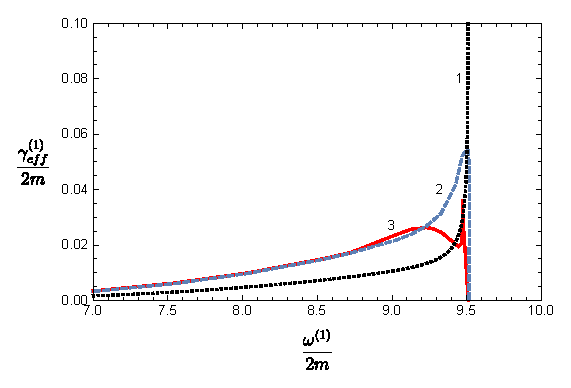
\includegraphics[scale=0.8]{mode1.eps}
	\caption{\label{fig:fig1}Зависимость ширины распада фотона моды 1 от частоты в припороговых областях при $B=200 B_e$, $T=1$ МэВ и $ \mu=0 $. Линия $ {\it 1} $ - коэффициент поглощения фотона $ W ^ {(1)}_{abs} $,
		% в процессах $ \ gamma \ to e ^ + e ^ - $ и $ \ gamma e ^ { \ pm} \ to e ^ {\ pm} $,
		вычисленный в древесном приближении и содержащий корневые особенности; линия $ {\it 2} $ - ширина распада, полученная из комплексного решения дисперсионного уравнения на втором римановом листе~\cite{Shabad:1988}; линия $ {\it 3} $ соответствует ширине затухания $ \gamma^{(1)}$, вычисленной на основе приближения~(\ref{eq:ApproxA}).}\label{fig:DampMode1}
\end{figure}

\begin{figure}[t!]\centering
	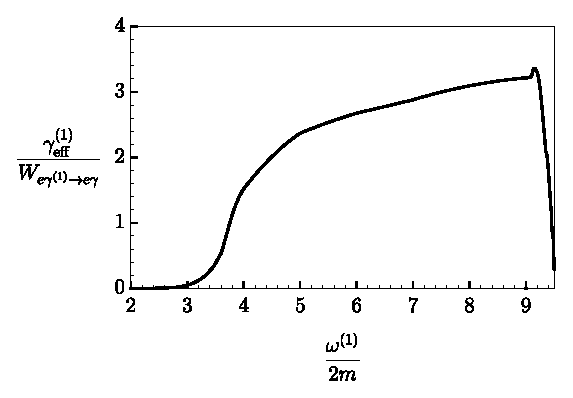
\includegraphics[scale=1.3]{CompareDampAndCompton.eps}
	\caption{\label{fig:ComptonandDamp} Отношение коэффициента затухания фотона $\gamma_{eff}^{(1)}$ к коэффициенту поглощения фотона в процессе $e\gamma^{(1)}\to e\gamma$ при $B=200B_e$ и $T=1$ МэВ}
\end{figure}
\clearpage
\begin{figure}[t!]\centering
	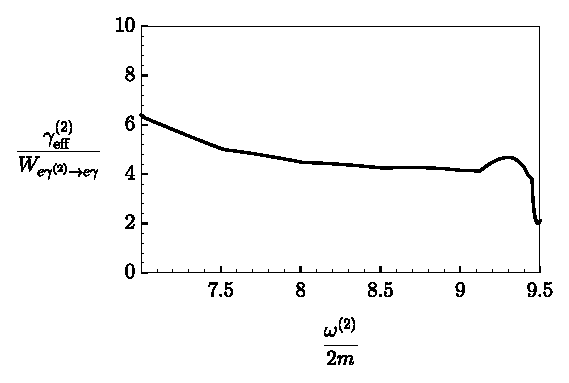
\includegraphics[scale=1.3]{CompareDampAndCompton2.eps}
	\caption{\label{fig:ComptonandDamp2} Отношение коэффициента затухания фотона $\gamma_\text{eff}^{(2)}$ к коэффициенту поглощения фотона в процессе $e\gamma^{(2)}\to e\gamma$ при $B=200B_e$ и $T=1$ МэВ}
\end{figure}


На основе полученных результатов представляет интерес рассмотреть задачу о 
возможности формирования комптоновского процесса при условии затухания фотона. 
Для этого удобно вычислить отношение коэффициента затухания фотона к 
коэффициенту поглощения фотона $e\gamma^{(1)}\to e\gamma$  (см. рис. 
\ref{fig:ComptonandDamp}), полученному в главе~\ref{sec:resonance} и 
определяющему время 
формирования процесса. Как видно из рисунка~\ref{fig:ComptonandDamp}, 
комптоновский 
процесс, несмотря на малый фактор $\alpha$, успевает формироваться при энергиях 
фотона $\omega\lesssim3$ МэВ. Для фотона моды 2 комптоновский процесс 
формируется только в области энергий фотона $\omega\lesssim1$ МэВ. В области 
энергий $\omega>3$ МэВ для моды 1 и $\omega>1$ МэВ для моды 2 фотоны будут 
эффективно 
затухать и комптоновский процесс, по-видимому, не успевает сформироваться. Для 
моды 2 (см. рис.~\ref{fig:ComptonandDamp2}) даже с учетом области 
квазистабильности (вдали от порогов), комптоновский процесс будет формироваться 
только при энергиях фотона~$\omega<1$~МэВ.

Таким образом, коэффициенты поглощения фотона в комптоновском процессе для двух 
возможных каналов рассеяния $e\gamma^{(1)}  \to e\gamma^{(1)}$ и 
$e\gamma^{(1)}  \to e\gamma^{(2)}$, несмотря на резонансный характер, 
целесообразно рассматривать лишь вдали от циклотронных резонансов, поэтому для 
анализа комптоновского процесса при высоких температурах $T\simeq 1$ МэВ и 
магнитных полях $B=200 B_e$ достаточно использовать разложение по обратным 
степеням напряженности магнитного поля~\cite{Chistyakov:2009}. Каналы  
рассеяния $e\gamma^{(2)}  \to e\gamma^{(1)}$  и $e\gamma^{(2)}  \to 
e\gamma^{(2)}$ в области резонанса рассматривать нецелесообразно, так как 
комптоновский процесс не успевает сформироваться для энергий фотона 
$\omega\gtrsim 2m$.

